\documentclass{beamer}
\usepackage{lmodern}

\usetheme{CambridgeUS} % try Madrid
\usecolortheme{beaver}
\usefonttheme[onlymath]{serif} % try "professionalfonts"

\setbeamertemplate{itemize items}[default]
\setbeamertemplate{enumerate items}[default]

\usepackage{amsmath, amsfonts, latexsym}
\DeclareMathOperator*{\argmin}{arg\,min}
\DeclareMathOperator*{\argmax}{arg\,max}

\usepackage{graphicx, subcaption}
\usepackage[normalem]{ulem}

% problem no.
\newcommand{\pno}[1]{\textcolor{blue}{\scriptsize [Problem: #1]}}
\newcommand{\set}[1]{\{#1\}}

%%%%%%%%%%%%%%%%%%%%
\title[Graph Decomposition]{Graph Decomposition}
\subtitle{--- DFS\&BFS, Cycle, DAG, SCC, and Biconnectivity}

\author[Hengfeng Wei]{}
\institute{hengxin0912@gmail.com}
\date{May 19, 2016}

\AtBeginSection[]{
  \begin{frame}[noframenumbering, plain]
    \frametitle{Graph Decomposition}
    \tableofcontents[currentsection, sectionstyle=show/shaded, subsectionstyle=show/show/hide]
  \end{frame}
}

% Delete this, if you do not want the table of contents to pop up 
% at the beginning of each subsection:
\AtBeginSubsection[]{
  \begin{frame}[noframenumbering, plain]
    \frametitle{Graph Decomposition}
      \tableofcontents[currentsection, sectionstyle=show/shaded, subsectionstyle=show/shaded/hide]
  \end{frame}
}

\begin{document}
\maketitle

\section{Overview}

\begin{frame}{Contents of Tutorials}
  \begin{enumerate}
    \item Graph \sout{Traversal} Decomposition
    \item MST (Greedy Algorithm) \& Path
    \item DP: Dynamic Programming
  \end{enumerate}
\end{frame}

\begin{frame}{Graph Decomposition}
  Graph decomposition vs. Graph traversal
\end{frame}

\section{DFS and BFS}

%%%%%%%%%%%%%%%%%%%%
\begin{frame}{Turing Award}
  \begin{columns}
	\column{0.50\textwidth}
	  \fignocaption{width = 0.40\textwidth}{figs/hopcroft.jpg}{\centerline{John Hopcroft}}
	\column{0.50\textwidth}
	  \fignocaption{width = 0.35\textwidth}{figs/tarjan.png}{\centerline{Robert Tarjan}}
  \end{columns}

  \vspace{0.50cm}
  \begin{quote}
	``For fundamental achievements in the design and analysis of algorithms and data structures.'' \\
	\hfill --- Turing Award, 1986
  \end{quote}
\end{frame}
%%%%%%%%%%%%%%%%%%%%
\begin{frame}{Depth-first search}
  \fignocaption{width = 0.55\textwidth}{figs/dfs-paper-tarjan}

  \uncover<2->{
	\begin{quote}
	  {\small ``We \textcolor{red}{have seen} how the depth-first search method may be used in the construction of
	  very efficient graph algorithms. $\dots$ \\
	  Depth-first search \textcolor{red}{is} a powerful technique with many applications.''}
	\end{quote}
  }

  \begin{alertblock}{Reference}
	\begin{itemize}
	  \item ``Depth-First Search And Linear Graph Algorithms'' by Robert Tarjan.
	\end{itemize}
  \end{alertblock}
\end{frame}
%%%%%%%%%%%%%%%%%%%%
\begin{frame}{Graph decomposition}
  \begin{center}
	Graph decomposition vs. Graph traversal \\[10pt]
	Structures!
  \end{center}

  \pause
  \begin{enumerate}
	\item states of vertices
	\item types of edges
	\item lifetime of vertices (DFS)
	  \begin{itemize}
	    \item $v: \text{d}[v], \text{f}[v]$
	    \item $\text{f}[v]$: DAG, SCC
	    \item $\text{d}[v]$: biconnectivity
	  \end{itemize}
  \end{enumerate}
\end{frame}
%%%%%%%%%%%%%%%%%%%%
\begin{frame}{Types of edges}
  \begin{definition}[Classifying edges]
    Given a DFS/BFS traversal $\Rightarrow$ DFS/BFS tree:
	\begin{description}[Forward edge:]
	  \item[Tree edge:] $\to$ child
	  \item[Back edge:] $\to$ ancestor
	  \item[Forward edge:] $\to$ \emph{nonchild} descendant
	  \item[Cross edge:] $\to$ neither ancestor nor descendant
    \end{description}
  \end{definition}

  \pause
  \begin{alertblock}{Remarks}
    \begin{itemize}
      \item applicable to both DFS and BFS
      \item w.r.t. DFS/BFS trees
    \end{itemize}
  \end{alertblock}
\end{frame}
%%%%%%%%%%%%%%%%%%%%
\begin{frame}{Types of edges (Problem 5.18)}
  \begin{figure}
	\begin{subfigure}{0.50\linewidth}
	  \centering
	  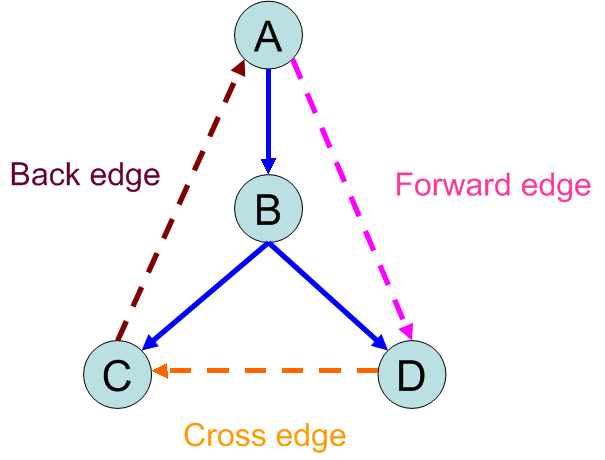
\includegraphics[width=0.50\textwidth]{figs/dfs-digraph.png}
	  \caption{DFS on directed graph.}
	\end{subfigure}%
	\begin{subfigure}{0.50\linewidth}
	  \centering
	  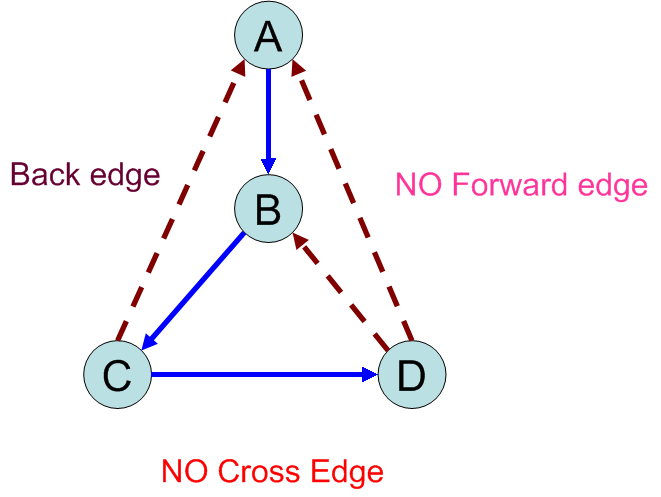
\includegraphics[width=0.50\textwidth]{figs/dfs-undirected.png}
	  \caption{DFS on undirected graph.}
	\end{subfigure}

	\begin{subfigure}{0.50\linewidth}
	  \centering
	  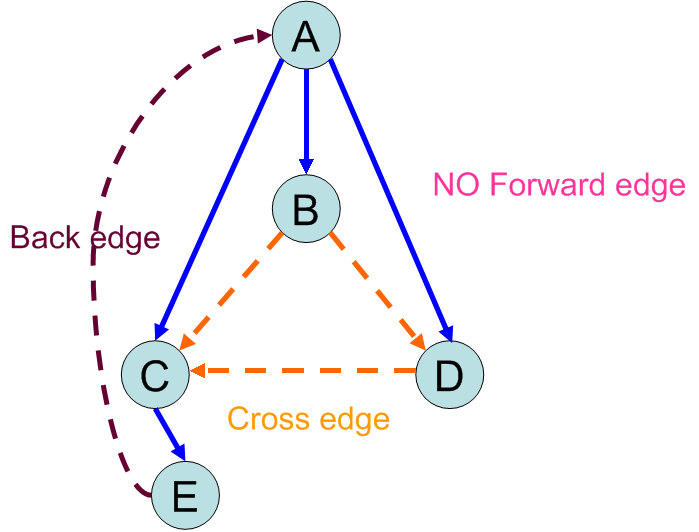
\includegraphics[width=0.50\textwidth]{figs/bfs-digraph.png}
	  \caption{BFS on directed graph.}
	\end{subfigure}%
	\begin{subfigure}{0.50\linewidth}
	  \centering
	  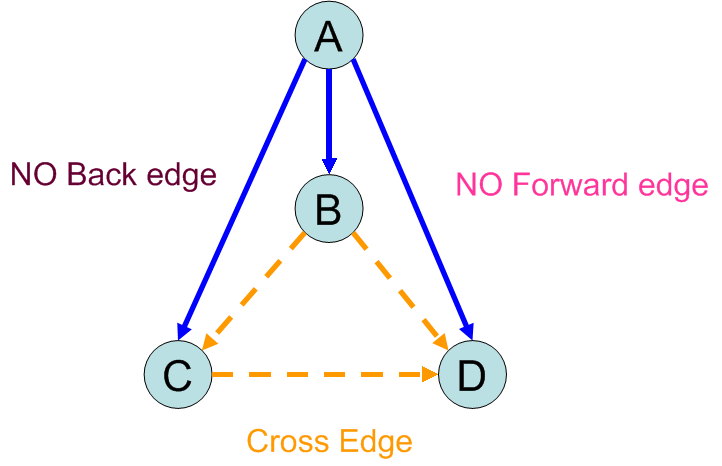
\includegraphics[width=0.60\textwidth]{figs/bfs-undirected.png}
	  \caption{BFS on undirected graph.}
	\end{subfigure}
  \end{figure}
\end{frame}
%%%%%%%%%%%%%%%%%%%%
\begin{frame}{Types of edges}
  \begin{exampleblock}{DFS tree and BFS tree coincide (Additional)}
    $G = (V,E), v \in V$. \\
	DFS tree $T$ = BFS tree $T'$.

    \begin{itemize}
      \item $G$ is an undirected graph $\implies G = T$
      \item $G$ is a digraph $\xLongrightarrow{?} G = T$
    \end{itemize}
  \end{exampleblock}

  \pause
  \begin{itemize}
	\item $T$: tree + back \emph{vs.} $T'$: tree + cross
	\pause
	\item $T$: tree + back + forward + cross \emph{vs.} $T'$: tree + back + cross 
  \end{itemize}
\end{frame}
%%%%%%%%%%%%%%%%%%%%
\begin{frame}{Lifttime of vertices in DFS}
  \begin{theorem}[Disjoint or contained]
	\begin{gather*}
	  \forall u,v: \\
	  [_{u} \; ]_{u} \cap [_{v} \; ]_{v} = \emptyset \\
	  \bigvee \\
	  ([_{u} \; ]_{u} \subsetneqq [_{v} \; ]_{v} \lor [_{v} \; ]_{v} \subsetneqq [_{u} \; ]_{u})
	\end{gather*}
  \end{theorem}

  \pause

  \begin{proof}
	\fignocaption{width = 0.30\textwidth}{figs/stack.png}
  \end{proof}
\end{frame}
%%%%%%%%%%%%%%%%%%%%
\begin{frame}{Ancestor/descendant relation}
  \begin{exampleblock}{Preprocessing for ancestor/descendant relation (Problem 5.23)}
    \begin{itemize}
      \item binary tree $T = (V, E)$ (tree)
      \item $r \in V$
    \end{itemize}
  \end{exampleblock}

  \[
	v: \text{d}[v], \text{f}[v]
  \]

  \pause
  \begin{alertblock}{Question}
    $\forall v$: how many descendants?

	\pause
    \[
	  (\text{f}[v] - \text{d}[v] - 1) / 2
	\]
  \end{alertblock}
\end{frame}
%%%%%%%%%%%%%%%%%%%%
\begin{frame}{Edge types and lifetime of vertices in DFS}
  \begin{exampleblock}{Edge types and lifetime of vertices in DFS (Problem 5.2)}
    $\forall u \to v$:
    \begin{itemize}
      \item tree/forward edge: $[_{u}\; [_{v}\; ]_{v}\; ]_{u}$
      \item back edge: $[_{v}\; [_{u}\; ]_{u}\; ]_{v}$
      \item cross edge: $[_{v}\; ]_{v}\; [_{u}\; ]_{u}$
    \end{itemize}
  \end{exampleblock}

  \pause

  \begin{alertblock}{Remark}
    \begin{itemize}
      \item $\text{f}[v] < \text{d}[u]$: cross edge
      \item $\text{f}[u] < \text{f}[v]$: back edge
		\pause
		\[
		  u \to v \iff \text{f}[v] < \text{f}[u]
		\]
    \end{itemize}
  \end{alertblock}
\end{frame}
%%%%%%%%%%%%%%%%%%%%
\begin{frame}{Height and diameter of tree}
  \begin{exampleblock}{Height and diameter of tree (Problem 5.21)}
	Binary tree $T = (V, E)$ with $|V| = n$:
	\begin{itemize}
	  \item height ($O(n)$)
	  \item diameter ($O(n)$)
	\end{itemize}
  \end{exampleblock}

  \begin{alertblock}{Question}
	Diameter of a tree \emph{without} designated root?
  \end{alertblock}
\end{frame}
%%%%%%%%%%%%%%%%%%%%
\begin{frame}{Perfect subtree}
  \begin{exampleblock}{Perfect subtree (Problem 5.22)}
	\begin{itemize}
	  \item binary tree $T = (V, E)$
	  \item root $r \in V$
	  \item goal: find all perfect subtrees
	\end{itemize}
  \end{exampleblock}
\end{frame}
%%%%%%%%%%%%%%%%%%%%
\begin{frame}{Counting shortest paths}
  \begin{exampleblock}{Counting shortest paths (Problem 5.26)}
  \end{exampleblock}
\end{frame}
%%%%%%%%%%%%%%%%%%%%

\section{Cycles}

%%%%%%%%%%%%%%%%%%%%
\begin{frame}{Cycle detection}
  \begin{exampleblock}{Cycle detection (Problem 5.24)}
	\begin{table}[ht]
	  \centering
	  \renewcommand{\arraystretch}{1.1}
	  \begin{tabular}{c||c|c}
	    \hline
		& Digraph 			& Undirected graph  \\ \hline \hline
		DFS & {\uncover<2->{back edge $\iff$ cycle}}
		& {\uncover<3->{back edge $\iff$ cycle}}
		\\ \hline
		BFS & {\uncover<5->{\begin{tabular}[c]{@{}l@{}}back edge $\implies$ cycle\\ cycle \textcolor{red}{$\centernot\implies$} back edge \end{tabular}}}
		& {\uncover<4->{cross edge $\iff$ cycle}}
		\\ \hline
	  \end{tabular}
	\end{table}
  \end{exampleblock}

  \begin{columns}
	\column{0.50\textwidth}
	  \uncover<6->{\fignocaption{width = 0.30\textwidth}{figs/bfs-digraph-cycle-without-back.png}}
	\column{0.50\textwidth}
	  \uncover<7->{%
		\begin{alertblock}{Remark}
		  How to identify back edges?
		\end{alertblock}}
  \end{columns}
\end{frame}
%%%%%%%%%%%%%%%%%%%%
\begin{frame}{Edge deletion}
  \begin{exampleblock}{Edge deletion (Problem 5.20)}
    \begin{itemize}
      \item connected, undirected graph $G$
      \item $\exists? e \in E: G \setminus e$ is connected?
      \item $O(|V|)$
    \end{itemize}
  \end{exampleblock}

  \pause
  \[
	\exists \text{ cycle} \iff \exists \text{ such } e
  \]

  \pause
  \[
	\text{tree: } |E| = |V| - 1 \implies \text{ check } |E| \ge |V|
  \]
\end{frame}
%%%%%%%%%%%%%%%%%%%%
\begin{frame}{Orientation of undirected graph}
  \begin{exampleblock}{Orientation of undirected graph (Problem 5.9)}
	\begin{itemize}
      \item undirected (connected) graph $G$ 
	  \item edges oriented \emph{s.t.} 
		\[
		  \forall v, \text{in}[v] \ge 1
		\]
	\end{itemize}
  \end{exampleblock}

  \pause
  \[
	\text{orientation} \iff \exists \text{ cycle } C
  \]

  \pause
  \[
	\text{BFS/DFS from } v \in C
  \]
\end{frame}
%%%%%%%%%%%%%%%%%%%%
\begin{frame}{Shortest cycle of undirected graph}
  \begin{exampleblock}{Shortest cycle of undirected graph (Problem 5.8)}
	Shortest cycle of $G$:
	\begin{itemize}
	  \item DFS on $G$
	  \item $\forall v: \text{level}[v]$
	  \item back edge $u \to v: \text{level}[u] - \text{level}[v] + 1$
	\end{itemize}
  \end{exampleblock}

  \pause
  \begin{alertblock}{Question}
	What about digraphs?
  \end{alertblock}
\end{frame}
%%%%%%%%%%%%%%%%%%%%

\section{DAG}

%%%%%%%%%%%%%%%%%%%%
\begin{frame}{DAG}
  \begin{center}
    no back edge $\iff$ DAG \pause $\iff$ $\exists$ topo. ordering
  \end{center}

  \begin{block}{Toposort algorithm by Tarjan (probably), 1976}
    DFS on digraph, $u \to v$:
    \begin{itemize}
	  \item \sout{back edge:} $\text{f}[u] < \text{f}[v]$
      \item others: $\text{f}[u] > \text{f}[v]$
    \end{itemize}

	\pause
    \[ 
	  u \to v \implies \text{f}[u] > \text{f}[v]
	\]

	\pause
    \begin{center}
	  Toposort: sort vertices in \textcolor{blue}{\emph{decreasing}} order of their \textcolor{blue}{\emph{finish}} times.
    \end{center}
  \end{block}
\end{frame}
%%%%%%%%%%%%%%%%%%%%
\begin{frame}{Kahn's toposort algorithm}
  \begin{exampleblock}{Kahn's toposort algorithm (1962; Problem 5.11) }
    \begin{itemize}
      \item queue for source vertices ($\text{in}[v] = 0$)
      \item repeat: dequeue $v$, delete it, output it
    \end{itemize}
  \end{exampleblock}

  \pause
  \begin{lemma}
	Every DAG has at least one source (and at least one sink vertex).
  \end{lemma}

  \pause
  \begin{alertblock}{Question}
	What if $G$ is not a DAG?
  \end{alertblock}
\end{frame}
%%%%%%%%%%%%%%%%%%%%
\begin{frame}{Taking courses}
  \begin{exampleblock}{Taking courses in few semesters (Problem 5.14)}
	\begin{itemize}
	  \item $n$ courses
	  \item $c_1 \to c_2$
	  \item goal: taking courses in few semesters
	\end{itemize}
  \end{exampleblock}

  \pause
  \begin{center}
	critical path \emph{OR} longest path
  \end{center}

  \pause
  \begin{alertblock}{Remark}
	For general digraph, LONGEST-PATH is NP-hard.
  \end{alertblock}
\end{frame}
%%%%%%%%%%%%%%%%%%%%
\begin{frame}{Line up}
  \begin{exampleblock}{Line up (Problem 5.16)}
    \begin{enumerate}
      \item $i$ hates $j$: $i \prec j$
      \item $i$ hates $j$: $\# i < \# j$
    \end{enumerate}
  \end{exampleblock}
\end{frame}
%%%%%%%%%%%%%%%%%%%%
\begin{frame}{Hamiltonian path in DAG}
  \begin{exampleblock}{Hamiltonian path in DAG (Problem 5.10)}
    \begin{itemize}
      \item DAG $G$
      \item HP: path visiting each vertex once
    \end{itemize}
  \end{exampleblock}

  \pause
  \begin{alertblock}{Remark}
    For general (di)graph, HP is NP-hard.
  \end{alertblock}

  \pause
  \[
	\text{DAG: } \exists \text{ HP} \iff \exists! \text{ topo. ordering}
  \]

  \begin{columns}
	\column{0.50\textwidth}
	  \pause
	  \begin{proof}
		$\Longleftarrow$: By contradiction. 
	  \end{proof}
	\column{0.50\textwidth}
	  \pause
	  Algorithms:
	  \begin{enumerate}
		\item toposort, check edges
		\item the Kahn toposort algorithm
	  \end{enumerate}
	\end{columns}
\end{frame}
%%%%%%%%%%%%%%%%%%%%


\end{document}
